\documentclass{article}


%\usepackage[latin1]{inputenc}
%\usepackage[spanish]{babel}

\usepackage{graphicx}
%\usepackage{psfig}
\usepackage{color}
\usepackage{url}
\usepackage{fancyhdr}
\usepackage{verbatim}

% Para que latex2html intreprete \htmladdnormallink 
\usepackage{html}

% Para que \htmladdnormallink se convierta a enlaces en el pdf
\usepackage{hyperref}

% Pijer�as varias con verbatim:
%	-> Podemos especificar el tipo, tama�o y estilo de letra a usar
%	-> Entiende los tabuladores...
\usepackage{fancyvrb}

% Macro para definir opciones al entorno Verbatim.
% Definimos una letra m�s peque�a que la que usa por defecto
% LaTeX para los entornos verbatim. 
\fvset{fontsize=\small,tabsize=3}

\newcommand{\ejemplo}[1]{
	\verbatiminput{#1}
}

%\newcommand{\ejemplo}[3]{
%	\VerbatimInput[
%			fontsize=\footnotesize,		% Tama�o de la fuente
%			frame=lines,					% Borde
%			framesep=2mm,					% Separaci�n del borde al texto
%			label=#3							% Etiqueta
%			]{#1}
%	\label{#2}
%}

% Comando que introducir� en el texto un cuadro con c�digo.
\newcommand{\codigo}[3]{
	\VerbatimInput[
			fontsize=\footnotesize,		% Tama�o de la fuente
			frame=lines,					% Borde
			framesep=2mm,					% Separaci�n del borde al texto
			numbers=left,					% N�meraci�n de l�neas
			label=#3							% Etiqueta
			]{#1}
	\label{#2}
}

% Comando que introducir� en el texto un cuadro con c�digo. Adem�s
% permite especificar unos l�mites: primera l�nea a mostrar y �ltima 
% l�nea a mostrar del archivo.
\newcommand{\codigowl}[4]{
	\VerbatimInput[
			fontsize=\footnotesize,		% Tama�o de la fuente
			frame=lines,					% Borde
			framesep=2mm,					% Separaci�n del borde al texto
			numbers=left,					% N�meraci�n de l�neas
			label=#1,						% Etiqueta
			firstline=#3,
			lastline=#4
			]{#2}
}

% Comando para introducir una imagen...
% Ejemplo: \figura{width=\textwidth}{imgs/prueba.eps}{img::prueba}{Una imagen de prueba}
\newcommand{\figura}[4]{
   \begin{figure}[htbp]
      \begin{center}
         \includegraphics[#1]{#2}
      \end{center}
      \caption{#4}
      \label{#3}
   \end{figure}
}

\frenchspacing


\author{Angel de Vicente}

\title{Hands-on session with Condor: Workbook}

\begin{document}

\maketitle
\thispagestyle{empty}
%\end{titlepage}

\tableofcontents

\newpage

\section{Preliminary}

The goal of this hands-on session is to gain experience with the main Condor
functions, understand the limits of Condor and how to solve problems if these
arise. In order to follow this session, you are supposed to have attended the
introductory talk on Condor given by Adrian Santos Marreros or at least have
read his presentation slides

(\htmladdnormallink{http://goya/inves/SINFIN/Condor/presentacion/presentacion\_condor.pdf}{http://goya/inves/SINFIN/Condor/presentacion/presentacion\_condor.pdf})
or the basic Condor instructions

(\htmladdnormallink{http://goya/inves/SINFIN/Condor/iac\_manual/manual.pdf}{http://goya/inves/SINFIN/Condor/iac\_manual/manual.pdf}). It
is assumed that you understand the basic concepts of Condor (what it is and why
it can be useful to you).


\section{Introduction}

Condor is developed by the Condor Team at the University of Wisconsin-Madison
(UW-Madison), and was first installed as a production system in the UW-Madison
Computer Sciences department more than 10 years ago.

In a nutshell, Condor is a specialized batch system for managing
compute-intensive jobs. Like most batch systems, Condor provides a queuing
mechanism, scheduling policy, priority scheme, and resource
classifications. Users submit their compute jobs to Condor, Condor puts the jobs
in a queue, runs them, and then informs the user as to the result.

Batch systems normally operate only with dedicated machines. Often termed
compute servers, these dedicated machines are typically owned by one
organization and dedicated to the sole purpose of running compute jobs. Condor
can schedule jobs on dedicated machines. But unlike traditional batch systems,
Condor is also designed to effectively utilize non-dedicated machines to run
jobs. By being told to only run compute jobs on machines which are currently not
being used (no keyboard activity, no load average, no active telnet users, etc),
Condor can effectively harness otherwise idle machines throughout a pool of
machines. This is important because often times the amount of compute power
represented by the aggregate total of all the non-dedicated desktop workstations
sitting on people's desks throughout the organization is far greater than the
compute power of a dedicated central resource.

\subsection{Getting to know the IAC Condor Pool}

Before we run anything with Condor, we need to find out what resources are available
at our pool. For this, we can use CondorView to view historical data, or
condor\_status to find about the current state of our pool.

\subsubsection{CondorView statistics}

This is a very easy-to-use web application that let's you see through time how many machines were in our
pool, how many were being used by Condor, who submitted jobs to the
pool, etc.

At present the CondorView interface is at
\htmladdnormallink{http://guinda.ll.iac.es:8080/Condor/}{http://guinda.ll.iac.es:8080/Condor/},
accessible through the IAC Condor page at 
\htmladdnormallink{http://goya/inves/SINFIN/Condor/}{http://goya/inves/SINFIN/Condor/}.


\subsubsection{The  condor\_status command}

\paragraph{The concept of matchmaking: ads in Condor.}

Before you learn how to submit a job, it is important to understand how
Condor allocates resources. Condor simplifies job submission by acting as a
matchmaker of ClassAds. Condor's ClassAds are analogous to the classified
advertising section of the newspaper. Sellers advertise specifics about what
they have to sell, hoping to attract a buyer. Buyers may advertise specifics
about what they wish to purchase. Both buyers and sellers list constraints that
need to be satisfied. In Condor, users submitting jobs can be thought of as
buyers of compute resources and machine owners are sellers.

All machines in a Condor pool advertise their attributes, such as available RAM
memory, CPU type and speed, virtual memory size, current load average, along
with other static and dynamic properties. This machine ClassAd also advertises
under what conditions it is willing to run a Condor job and what type of job it
would prefer. You may advertise that your machine is only willing to run jobs at
night and when there is no keyboard activity on your machine. In addition, you
may advertise a preference (rank) for running jobs submitted by you or one of
your co-workers.

Likewise, when submitting a job, you specify a ClassAd with your requirements
and preferences. The ClassAd includes the type of machine you wish to use. For
instance, perhaps you are looking for the fastest floating point performance
available. You want Condor to rank available machines based upon floating point
performance. Or, perhaps you care only that the machine has a minimum of 128
Mbytes of RAM. 

Condor plays the role of a matchmaker by continuously reading all the job
ClassAds and all the machine ClassAds, matching and ranking job ads with machine
ads. Condor makes certain that all requirements in both ClassAds are satisfied.

\paragraph{Inspecting Machine ClassAds with condor\_status.}

Once Condor is installed, you will get a feel for what a machine ClassAd does by
trying the condor\_status command. 

\begin{verbatim}
naranja(67)~/Condor-Course/dagman1> condor_status

Name          OpSys       Arch   State      Activity   LoadAv Mem   ActvtyTime

canistel.iac. LINUX       INTEL  Claimed    Suspended  0.800   500  0+00:00:04
codorniz.iac. LINUX       INTEL  Owner      Idle       5.000   500  0+19:25:20
correhuela.ia LINUX       INTEL  Claimed    Suspended  0.830  1005  0+00:00:04
drosera.iac.e LINUX       INTEL  Claimed    Suspended  0.830   248  0+00:00:04
paraguayo.iac LINUX       INTEL  Owner      Idle       0.000   500  0+00:50:04
resines.ll.ia LINUX       INTEL  Owner      Idle       3.030  1005  0+04:13:10
temple.ll.iac LINUX       INTEL  Owner      Idle       2.000   500  0+04:16:09
abeto.iac.es  SOLARIS29   SUN4u  Claimed    Suspended  0.420   256  0+00:02:00
aguila.iac.es SOLARIS29   SUN4u  Owner      Idle       0.050   640  0+01:18:55
ajedrea.iac.e SOLARIS29   SUN4u  Claimed    Busy       1.000   512  0+19:00:42
albatros.iac. SOLARIS29   SUN4u  Claimed    Suspended  0.090   640  0+00:00:04
anchoa.ll.iac SOLARIS29   SUN4u  Claimed    Busy       1.000   256  0+19:13:47
ansar.iac.es  SOLARIS29   SUN4u  Claimed    Busy       1.000   576  0+15:35:16
asno.iac.es   SOLARIS29   SUN4u  Claimed    Busy       1.020   256  0+01:00:53
avestruz.iac. SOLARIS29   SUN4u  Claimed    Busy       0.990   128  0+17:51:11
[...]

                     Machines Owner Claimed Unclaimed Matched Preempting

         INTEL/LINUX        7     4       3         0       0          0
     SUN4u/SOLARIS29       94    26      68         0       0          0

               Total      101    30      71         0       0          0
naranja(68)~/Condor-Course/dagman1>
\end{verbatim}

But there is much more to condor\_status\dots Here there are some useful options
of the condor\_status command:

\begin{itemize}
\item Show only machines which are willing to run jobs now: \begin{verbatim}condor_status -available\end{verbatim}
\item Show only machines which are currently running jobs: \begin{verbatim}condor_status -run\end{verbatim}
\item Show all the machines in the pool sorted by the amount of memory they
  have: \begin{verbatim}condor_status -sort Memory\end{verbatim}
\item List the machine ClassAds for a given machines in the pool:
  \begin{verbatim}condor_status -l codorniz.iac.es 

For example:

naranja(68)~/Condor-Course/dagman1> condor_status -l naranja.iac.es
MyType = "Machine"
TargetType = "Job"
Name = "naranja.iac.es"
Machine = "naranja.iac.es"
Rank = 0.000000
CpuBusy = ((LoadAvg - CondorLoadAvg) >= 0.500000)
COLLECTOR_HOST_STRING = "codorniz"
CondorVersion = "$CondorVersion: 6.6.3 Mar 29 2004 $"
CondorPlatform = "$CondorPlatform: SUN4X-SOLARIS29 $"
VirtualMachineID = 1
ExecutableSize = 284
JobUniverse = 5
NiceUser = FALSE
ImageSize = 8304
VirtualMemory = 384888
Disk = 30672106
CondorLoadAvg = 0.940000
LoadAvg = 0.940000
KeyboardIdle = 1
ConsoleIdle = 60233
Memory = 640
Cpus = 1
StartdIpAddr = "<161.72.64.97:62302>"
Arch = "SUN4u"
OpSys = "SOLARIS29"
UidDomain = "iac.es"
FileSystemDomain = "iac.es"
Subnet = "161.72.64"
HasIOProxy = TRUE
TotalVirtualMemory = 384888
TotalDisk = 30672106
KFlops = 102016
Mips = 601
LastBenchmark = 1096346012
TotalLoadAvg = 0.940000
TotalCondorLoadAvg = 0.940000
ClockMin = 671
ClockDay = 2
TotalVirtualMachines = 1
HasFileTransfer = TRUE
HasMPI = TRUE
HasJICLocalConfig = TRUE
HasJICLocalStdin = TRUE
JavaVendor = "Sun Microsystems Inc."
JavaVersion = "1.4.1_01a"
JavaMFlops = 15.282580
HasJava = TRUE
HasRemoteSyscalls = TRUE
HasCheckpointing = TRUE
StarterAbilityList = "HasFileTransfer,HasMPI,HasJICLocalConfig,HasJICLocalStdin,
                      HasJava,HasRemoteSyscalls,HasCheckpointing"
CpuBusyTime = 0
CpuIsBusy = FALSE
State = "Claimed"
EnteredCurrentState = 1096364649
Activity = "Suspended"
EnteredCurrentActivity = 1096366304
Start = ((KeyboardIdle > 15 * 60) && (((LoadAvg - CondorLoadAvg) <= 0.300000) || 
                                       (State != "Unclaimed" && State != "Owner")))
Requirements = START
CurrentRank = 0.000000
RemoteUser = "plopez@iac.es"
RemoteOwner = "plopez@iac.es"
ClientMachine = "naranja.iac.es"
JobId = "3362.0"
JobStart = 1096364653

[...]

DaemonStartTime = 1096054048
UpdateSequenceNumber = 1087
MyAddress = "<161.72.64.97:62302>"
LastHeardFrom = 1096366308
UpdatesTotal = 247
UpdatesSequenced = 246
UpdatesLost = 3
UpdatesHistory = "0x04400000000000000000000000000000"


naranja(69)~/Condor-Course/dagman1>
\end{verbatim}

\end{itemize}

Some of the listed attributes are used by Condor for scheduling. Other
attributes are for information purposes. An important point is that any of the
attributes in a machine ad can be utilized at job submission time as part of a
request or preference on what machine to use. Additional attributes can be
easily added. For example, your site administrator can add a physical location
attribute to your machine ClassAds.

\subsubsection{Exercises}
\label{ex_condor_status}
Refer to the condor\_status command reference page (section 9 of the Condor
manual \htmladdnormallink{http://goya/inves/SINFIN/Condor/v6.6/}{http://goya/inves/SINFIN/Condor/v6.6/}) to find out how to obtain the
following information:

\begin{enumerate}
\item A list of all the Linux machines available, sorted by their amount
  of memory.
\item A list of the java version installed in all the Java-capable Solaris
  machines (printed in the format given below), using only one condor\_status command:

\begin{verbatim}
The machine toro.iac.es has Java Version: 1.4.1_01a
The machine vibora.iac.es has Java Version: 1.4.1_01a
The machine viola.iac.es has Java Version: 1.4.1_01a
The machine zorro.ll.iac.es has Java Version: 1.4.1_01a
[...]
\end{verbatim}

\end{enumerate}




\section{Basic job submission}

\subsection{Before we start: road-map for running jobs}

The road to using Condor effectively is a short one. The basics are quickly and
easily learned. Here are the four steps needed to run a job using Condor:

\begin{enumerate}
\item \textbf{Prepare your code.}
    A job run under Condor must be able to run as a background batch job. Condor
runs the program unattended and in the background. A program that runs in the
background will not be able to do interactive input and output. Condor can
redirect console output (stdout and stderr) and keyboard input (stdin) to and
from files for you. Create any needed files that contain the proper keystrokes
needed for program input. Make certain the program will run correctly with the
files.

\item \textbf{Choose a Condor Universe.}
 Condor has several runtime environments (called a universe) from which to
 choose. For the moment we will start with the less restrictive one, the vanilla
 universe, and we'll worry about the other universes later on.

\item \textbf{Write the submit description file.}  
Controlling the details of a job submission is a submit description file. The
file contains information about the job such as what executable to run, the
files to use for keyboard and screen data, the platform type required to run the
program, and where to send e-mail when the job completes. You can also tell
Condor how many times to run a program; it is simple to run the same program
multiple times with multiple data sets.

\item \textbf{Submit the Job.}
Submit the program to Condor with the condor\_submit command. Once submitted,
Condor does the rest toward running the job. Monitor the job's progress with the
condor\_q and condor\_status commands. You may modify the order in which Condor
will run your jobs with condor\_prio. If desired, Condor can even inform you in
a log file every time your job is checkpointed and/or migrated to a different
machine.

When your program completes, Condor will tell you (by e-mail, if preferred) the
exit status of your program and various statistics about its performances,
including time used and I/O performed. If you are using a log file for the
job (which is recommended) the exit status will be recorded in the log file. You
can remove a job from the queue prematurely with condor\_rm.

Let's try it out\dots
\end{enumerate}

\subsection{The simplest job.}

\textit{In order to follow the examples and exercises, make sure you have
  created the following directories in your machine:}

\begin{itemize}
\item /home/$<$username$>$/Condor-Course
\item /scratch/Condor-Course
\end{itemize}

\textit{The code for all the examples and the exercises in this workbook are
  available from the IAC Condor page at
  \htmladdnormallink{http://goya/inves/SINFIN/Condor/}{http://goya/inves/SINFIN/Condor/},
  and you should copy them to Condor-Course in your home directory.}

\subsubsection{Example}

\paragraph{Submission file}

\begin{verbatim}
########################################################
##
## Example 1
##
## Simple condor job description file
##
########################################################

executable = /bin/uname
universe = vanilla
output = example1.out
error =  example1.err
log =    example1.log
queue
\end{verbatim}

\paragraph{Running example}

\begin{verbatim}
[angelv@guinda ~/Condor-Course]$ condor_submit example1.submit 
Submitting job(s).
Logging submit event(s).
1 job(s) submitted to cluster 172.


[angelv@guinda ~/Condor-Course]$ condor_q
-- Submitter: guinda.iac.es : <161.72.81.187:32795> : guinda.iac.es
 ID      OWNER            SUBMITTED     RUN_TIME ST PRI SIZE CMD               
 172.0   angelv          9/22 16:41   0+00:00:01 R  0   0.0  uname             

1 jobs; 0 idle, 1 running, 0 held


[angelv@guinda ~/Condor-Course]$ condor_q
-- Submitter: guinda.iac.es : <161.72.81.187:32795> : guinda.iac.es
 ID      OWNER            SUBMITTED     RUN_TIME ST PRI SIZE CMD               

0 jobs; 0 idle, 0 running, 0 held


[angelv@guinda ~/Condor-Course]$ cat example1.out 
Linux


[angelv@guinda ~/Condor-Course]$ cat example1.err


[angelv@guinda ~/Condor-Course]$ cat example1.log 
000 (172.000.000) 09/22 16:41:08 Job submitted from host: <161.72.81.187:32795>
...
001 (172.000.000) 09/22 16:41:14 Job executing on host: <161.72.80.28:56778>
...
005 (172.000.000) 09/22 16:41:14 Job terminated.
	(1) Normal termination (return value 0)
		Usr 0 00:00:00, Sys 0 00:00:00  -  Run Remote Usage
		Usr 0 00:00:00, Sys 0 00:00:00  -  Run Local Usage
		Usr 0 00:00:00, Sys 0 00:00:00  -  Total Remote Usage
		Usr 0 00:00:00, Sys 0 00:00:00  -  Total Local Usage
	0  -  Run Bytes Sent By Job
	0  -  Run Bytes Received By Job
	0  -  Total Bytes Sent By Job
	0  -  Total Bytes Received By Job
...

[angelv@guinda ~/Condor-Course]$ host 161.72.80.28
28.80.72.161.in-addr.arpa domain name pointer canistel.ll.iac.es.

\end{verbatim}

\paragraph{Mail from Condor system.} Unless you specify not to, you will receive an e-mail from Condor when each of
your jobs completes or has any errors.

\begin{verbatim}
From: condor@iac.es (Condor Administrator)
To: angelv@iac.es
Subject: [Condor] Condor Job 172.0
Date: Wed, 22 Sep 2004 16:41:14 +0100 (WEST)

This is an automated email from the Condor system
on machine "guinda.iac.es".  Do not reply.

Your Condor job 172.0 
	/bin/uname 
has exited normally with status 0.


Submitted at:        Wed Sep 22 16:41:08 2004
Completed at:        Wed Sep 22 16:41:14 2004
Real Time:           0 00:00:06

Virtual Image Size:  12 Kilobytes

Statistics from last run:
Allocation/Run time:     0 00:00:02
Remote User CPU Time:    0 00:00:00
Remote System CPU Time:  0 00:00:00
Total Remote CPU Time:   0 00:00:00

Statistics totaled from all runs:
Allocation/Run time:     0 00:00:02

Network:
    0.0 B  Run Bytes Received By Job
    0.0 B  Run Bytes Sent By Job


-=-=-=-=-=-=-=-=-=-=-=-=-=-=-=-=-=-=-=-=-=
Questions about this message or Condor in general?
Email address of the local Condor administrator: condor@iac.es
The Official Condor Homepage is http://www.cs.wisc.edu/condor
\end{verbatim}

\subsubsection{Exercise}
\label{ex_disk_info}

Modify the example above, so that the executable instead of being a system
command will be a program written by you called disk\_info.sh. 

Write the code for disk\_info.sh. This is a basic shell script that using the
commands uname, df, and grep will find the available scratch space. 

Submit the job to Condor. The output should be similar to:

\begin{verbatim}
[angelv@guinda Exercises]$ cat exercise1.out
bicuda
/dev/hda3              70G   43G   24G  65% /scratch
/dev/hdb1             126G   54G   67G  45% /scratch1
[angelv@guinda Exercises]$
\end{verbatim}

\subsection{Did you get any errors?}

Congratulations if you got the previous exercise without errors, but it is
likely that the first times you submit jobs to Condor you will get into
trouble. A common error is problems accesing your code or data files. Below
there are two examples.

\subsubsection{Example}

\paragraph{Submission file}
\begin{verbatim}
########################################################
##
## Example 2
##
## Simple condor job description file (with errors)
##
########################################################

executable = uname
universe = vanilla
output = example2.out
error =  example2.err
log =    example2.log
queue
\end{verbatim}

\paragraph{Running the code.}

In this case, Condor will complain right away\dots

\begin{verbatim}
[angelv@guinda ~/Condor-Course]$ condor_submit example2.submit
Submitting job(s)
ERROR: failed to transfer executable file uname
\end{verbatim}


\subsubsection{Example}

\paragraph{Submission file}
\begin{verbatim}
########################################################
##
## Example 3
##
## Simple condor job description file (with errors)
##
########################################################

executable = /bin/uname
universe = vanilla
output = /scratch/angelv/Condor-Course/example3.out
error =  /scratch/angelv/Condor-Course/example3.err
log =    example3.log
queue
\end{verbatim}

\paragraph{Running the code.}

This case is more subtle. It will look like your job is put in the queue, it
will run for a while, and then it will be put in the idle state, and then back
to the running state, and so on\dots  In these cases the log file is your best
friend. 

\begin{verbatim}
[angelv@guinda ~/Condor-Course]$ ls -l /scratch/angelv/
total 16
drwxr-xr-x   14 angelv   games        4096 sep 16 14:39 Audio
drwxr-xr-x    2 angelv   games        4096 sep 22 16:50 Condor-Course
drwxr-xr-x    4 angelv   games        4096 dic 19  2003 Documentation
drwxrwxr-x   15 angelv   games        4096 sep  7 14:29 Work


[angelv@guinda ~/Condor-Course]$ condor_submit example3.submit
Submitting job(s).
Logging submit event(s).
1 job(s) submitted to cluster 174.

[angelv@guinda ~/Condor-Course]$ ls /scratch/angelv/Condor-Course/
example3.err  example3.out


[angelv@guinda ~/Condor-Course]$ cat /scratch/angelv/Condor-Course/example3.err 


[angelv@guinda ~/Condor-Course]$ cat /scratch/angelv/Condor-Course/example3.out


[angelv@guinda ~/Condor-Course]$ cat example3.log 
000 (174.000.000) 09/22 16:50:59 Job submitted from host: <161.72.81.187:32795>
...
007 (174.000.000) 09/22 16:51:19 Shadow exception!
	Error from starter on canistel.iac.es: Failed to open standard output file 
  '/scratch/angelv/Condor-Course/example3.out': No such file or directory (errno 2)
	0  -  Run Bytes Sent By Job
	0  -  Run Bytes Received By Job
...
007 (174.000.000) 09/22 16:51:21 Shadow exception!
	Error from starter on canistel.iac.es: Failed to open standard output file 
  '/scratch/angelv/Condor-Course/example3.out': No such file or directory (errno 2)
	0  -  Run Bytes Sent By Job
	0  -  Run Bytes Received By Job
...
007 (174.000.000) 09/22 16:51:23 Shadow exception!
	Error from starter on canistel.iac.es: Failed to open standard output file 
  '/scratch/angelv/Condor-Course/example3.out': No such file or directory (errno 2)
	0  -  Run Bytes Sent By Job
	0  -  Run Bytes Received By Job
...
\end{verbatim}


\subsection{Initialdir to the rescue\dots}

\subsubsection{Example}

\paragraph{Submission file}
\begin{verbatim}
########################################################
##
## Example 4
##
## Using Initialdir
##
########################################################

executable = /bin/uname
universe = vanilla

Initialdir = /net/guinda/scratch/angelv/Condor-Course/
output = example4.out
error =  example4.err
log =    example4.log
queue
\end{verbatim}

\paragraph{Running the code}
\begin{verbatim}
[angelv@guinda ~/Condor-Course]$ condor_submit example4.submit
Submitting job(s).
Logging submit event(s).
1 job(s) submitted to cluster 181.

[angelv@guinda ~/Condor-Course]$ ls /scratch/angelv/Condor-Course/
example4.err  example4.log  example4.out

[angelv@guinda ~/Condor-Course]$ cat /scratch/angelv/Condor-Course/example4.out
Linux
[angelv@guinda ~/Condor-Course]$
\end{verbatim}


\subsection{Now, let's get our hands dirty\dots}

Until now, we have only seen toy submission files! Let's see a much more
powerful example.

\subsubsection{Example}
\paragraph{Submission file}
\begin{verbatim}
########################################################
##
## Example 5
##
## A realistic submission file
##
########################################################

executable = mycode.$$(OpSys)
universe = vanilla
Requirements = Memory >= 1000 && ((Arch == "INTEL" && OpSys == "LINUX") || \ 
                                  (Arch == "SUN4u" && OpSys == "SOLARIS29"))
Rank = Memory


Initialdir = /net/guinda/scratch/angelv/Condor-Course/
arguments = $(Process)
output = example5.$(Process).out
error =  example5.$(Process).err
log =    example5.log
queue 20

------------------------------------------------------------------

#!/usr/bin/tcsh

# mycode.SOLARIS29

echo I yawn, therefore I will be sleeping $argv[1] seconds ...
sleep $argv[1]
echo This amazing program was run in `uname -n`, a `uname -m` on `date`

-------------------------------------------------------------------

#!/bin/tcsh

## mycode.LINUX

echo The argument you passed me is $argv[1], so I will be sleeping $argv[1] seconds ...
sleep $argv[1]
echo This amazing program was run in `uname -n`, a `uname -m` on `date`
\end{verbatim}

\paragraph{Running the code}
\begin{verbatim}
[angelv@guinda ~/Condor-Course]$ condor_status -constraint 'Memory >= 1000' \ 
-sort Memory -format "%s " Machine -format "%d \n"  Memory

codorniz.iac.es 1005
sandia.iac.es 1005
correhuela.iac.es 1005
hinojo.iac.es 1005
tiburon.iac.es 1005
durazno.iac.es 1005
ortiga.iac.es 1005
sargo.iac.es 1005
praca.iac.es 1005
melocoton.iac.es 1005
odiseo.iac.es 1005
botero.iac.es 1006
botero.iac.es 1006
camelia.iac.es 1006
camelia.iac.es 1006
faya.iac.es 1024
rex.iac.es 1024
rex.iac.es 1024
rex.iac.es 1024
rex.iac.es 1024
peje.iac.es 1024
cebra.iac.es 1024
choco.iac.es 1152
coco.iac.es 1510
rambutan.iac.es 1510
rambutan.iac.es 1510
tuno.iac.es 1510
agrimonia.iac.es 1826
agrimonia.iac.es 1826
orca.iac.es 2015
cobos.iac.es 2015
bicuda.iac.es 2015
trueno.iac.es 2015
[angelv@guinda ~/Condor-Course]$

[angelv@guinda ~/Condor-Course]$ condor_submit example5.submit
Submitting job(s)....................
Logging submit event(s)....................
20 job(s) submitted to cluster 183.
[angelv@guinda ~/Condor-Course]$

--------------------------------------------------------------

[angelv@guinda Condor-Course]$ pwd
/scratch/angelv/Condor-Course

[angelv@guinda Condor-Course]$ cat example5*out
The argument you passed me is 0, so I will be sleeping 0 seconds ...
This amazing program was run in cobos, a i686 on Wed Sep 29 15:23:28 WEST 2004
The argument you passed me is 10, so I will be sleeping 10 seconds ...
This amazing program was run in camelia, a i686 on Wed Sep 29 15:23:59 WEST 2004
The argument you passed me is 11, so I will be sleeping 11 seconds ...
This amazing program was run in camelia, a i686 on Wed Sep 29 15:24:03 WEST 2004
The argument you passed me is 12, so I will be sleeping 12 seconds ...
This amazing program was run in codorniz, a i686 on Wed Sep 29 15:24:00 WEST 2004
The argument you passed me is 13, so I will be sleeping 13 seconds ...
This amazing program was run in odiseo, a i686 on Wed Sep 29 15:24:06 WEST 2004
The argument you passed me is 14, so I will be sleeping 14 seconds ...
This amazing program was run in hinojo, a i686 on Wed Sep 29 15:24:09 WEST 2004
The argument you passed me is 15, so I will be sleeping 15 seconds ...
This amazing program was run in cobos, a i686 on Wed Sep 29 15:24:13 WEST 2004
The argument you passed me is 16, so I will be sleeping 16 seconds ...
This amazing program was run in trueno, a i686 on Wed Sep 29 15:24:15 WEST 2004
The argument you passed me is 17, so I will be sleeping 17 seconds ...
This amazing program was run in agrimonia, a i686 on Wed Sep 29 15:24:19 WEST 2004
The argument you passed me is 18, so I will be sleeping 18 seconds ...
This amazing program was run in agrimonia, a i686 on Wed Sep 29 15:24:21 WEST 2004
The argument you passed me is 19, so I will be sleeping 19 seconds ...
This amazing program was run in rambutan, a i686 on Wed Sep 29 15:24:44 WEST 2004
The argument you passed me is 1, so I will be sleeping 1 seconds ...
This amazing program was run in trueno, a i686 on Wed Sep 29 15:23:31 WEST 2004
The argument you passed me is 2, so I will be sleeping 2 seconds ...
This amazing program was run in agrimonia, a i686 on Wed Sep 29 15:23:34 WEST 2004
The argument you passed me is 3, so I will be sleeping 3 seconds ...
This amazing program was run in agrimonia, a i686 on Wed Sep 29 15:23:36 WEST 2004
The argument you passed me is 4, so I will be sleeping 4 seconds ...
This amazing program was run in rambutan, a i686 on Wed Sep 29 15:23:40 WEST 2004
The argument you passed me is 5, so I will be sleeping 5 seconds ...
This amazing program was run in rambutan, a i686 on Wed Sep 29 15:23:42 WEST 2004
The argument you passed me is 6, so I will be sleeping 6 seconds ...
This amazing program was run in coco, a i686 on Wed Sep 29 15:23:47 WEST 2004
I yawn, therefore I will be sleeping 7 seconds ...
This amazing program was run in faya, a sun4u on Wed Sep 29 15:23:51 WEST 2004
The argument you passed me is 8, so I will be sleeping 8 seconds ...
This amazing program was run in botero, a i686 on Wed Sep 29 15:23:48 WEST 2004
The argument you passed me is 9, so I will be sleeping 9 seconds ...
This amazing program was run in botero, a i686 on Wed Sep 29 15:23:54 WEST 2004
[angelv@guinda Condor-Course]$
\end{verbatim}


\subsubsection{Exercise}
\label{ex_R}

In the previous example, we have used the keyword ``arguments'' in order to
customize each run of the program. For this exercise we will use the keyword
``input'', which indicates a file that contains the standard input (i.e. what
you would normally type in the keyboard) for your program. 

For this, we are going to use the R statistical package, which is installed for
both Linux and Solaris. The test file \textit{test.R} contains:

\begin{verbatim}
2+2
q()
\end{verbatim}

These are the commands that you would type into R to do the unimaginative task
of adding 2 + 2 and quitting. You can try it out like this:

\begin{verbatim}
[angelv@guinda ~/Condor-Course]$ R --vanilla < test.R

R : Copyright 2003, The R Development Core Team
Version 1.8.0  (2003-10-08)

R is free software and comes with ABSOLUTELY NO WARRANTY.
You are welcome to redistribute it under certain conditions.
Type 'license()' or 'licence()' for distribution details.

R is a collaborative project with many contributors.
Type 'contributors()' for more information.

Type 'demo()' for some demos, 'help()' for on-line help, or
'help.start()' for a HTML browser interface to help.
Type 'q()' to quit R.

> 2+2
[1] 4
> q()
[angelv@guinda ~/Condor-Course]$
\end{verbatim}

Amazingly we get a 4 as the answer! Now, your task is to modify the previous
example and prepare a submission file that will run 2 jobs in R, one to
calculate 2+2 and another one to calculate 3+3.

\section{Managing jobs}
This section provides a brief summary of some other things that can be done
once jobs are submitted. The basic mechanisms for monitoring a job are
introduced, but the commands are discussed briefly. You are encouraged to look
at the man pages of the commands referred to for more information.

When jobs are submitted, Condor will attempt to find resources to run the
jobs. A list of all those with jobs submitted may be obtained through condor\_
status with the -submitters option. An example of this would yield output
similar to:

\begin{verbatim}
[angelv@guinda ~/Condor-Course]$ condor_status -submitters

Name                 Machine      Running IdleJobs HeldJobs

apadron@iac.es       cormoran.i         1        0        0
delgadom@iac.es      gladiolo.i         1        0        0
angelv@iac.es        guinda.iac         1        0        0
delgadom@iac.es      lila.iac.e        22       28        0
plopez@iac.es        naranja.ia        81       62        0
apadron@iac.es       rex.iac.es         0        0       24

                           RunningJobs           IdleJobs           HeldJobs

       angelv@iac.es                 1                  0                  0
      apadron@iac.es                 1                  0                 24
     delgadom@iac.es                23                 28                  0
       plopez@iac.es                81                 62                  0

               Total               106                 90                 24
\end{verbatim}


\subsection{Checking on the progress of jobs}

As we have seen, you can check on the status of your jobs with the condor\_q
command. The output contains many columns of information about the queued
jobs. The ST column (for status) shows the status of current jobs in the
queue. An R in the status column means the the job is currently running. An I
stands for idle. The job is not running right now, because it is waiting for a
machine to become available. The status H is the hold state. In the hold state,
the job will not be scheduled to run until it is released (see the condor\_hold
reference page and the condor\_release reference page).

To get more detailed information about the queued jobs, you can use the option
-l with condor\_q command.

\begin{verbatim}
[angelv@guinda ~]$ condor_q -l 3881.0

-- Schedd: naranja.iac.es : <161.72.64.97:33152>
MyType = "Job"
TargetType = "Machine"
ClusterId = 3881
QDate = 1097666845
CompletionDate = 0
Owner = "plopez"
RemoteWallClockTime = 0.000000
LocalUserCpu = 0.000000
LocalSysCpu = 0.000000
RemoteUserCpu = 0.000000
RemoteSysCpu = 0.000000
ExitStatus = 0
NumCkpts = 0
NumRestarts = 0
NumSystemHolds = 0
CommittedTime = 0
TotalSuspensions = 0
LastSuspensionTime = 0
CumulativeSuspensionTime = 0
ExitBySignal = FALSE
CondorVersion = "$CondorVersion: 6.6.3 Mar 29 2004 $"
CondorPlatform = "$CondorPlatform: SUN4X-SOLARIS29 $"
RootDir = "/"
Iwd = "/home/plopez/tmp/run_41/."
JobUniverse = 5
Cmd = "/home/plopez/tmp/run_41/../setiathome-3.03.sparcv9-sun-solaris2.7/setiathome"
MinHosts = 1
MaxHosts = 1
CurrentHosts = 0
WantRemoteSyscalls = FALSE
WantCheckpoint = FALSE
JobStatus = 1
EnteredCurrentStatus = 1097666845
JobPrio = 0
User = "plopez@iac.es"
NiceUser = FALSE
Env = ""
JobNotification = 0
UserLog = "/home/plopez/tmp/run_41/./results.log"

[...]

[angelv@guinda ~]$
\end{verbatim}

You can also find all the machines that are running your job through the
condor\_status command. For example, to find all the machines that are running
jobs submitted by ``breach@cs.wisc.edu,'' type:

\begin{verbatim}
%  condor_status -constraint 'RemoteUser == "breach@cs.wisc.edu"'

Name       Arch     OpSys        State      Activity   LoadAv Mem  ActvtyTime

alfred.cs. INTEL    SOLARIS251   Claimed    Busy       0.980  64    0+07:10:02
biron.cs.w INTEL    SOLARIS251   Claimed    Busy       1.000  128   0+01:10:00
cambridge. INTEL    SOLARIS251   Claimed    Busy       0.988  64    0+00:15:00
falcons.cs INTEL    SOLARIS251   Claimed    Busy       0.996  32    0+02:05:03
happy.cs.w INTEL    SOLARIS251   Claimed    Busy       0.988  128   0+03:05:00
istat03.st INTEL    SOLARIS251   Claimed    Busy       0.883  64    0+06:45:01
istat04.st INTEL    SOLARIS251   Claimed    Busy       0.988  64    0+00:10:00
istat09.st INTEL    SOLARIS251   Claimed    Busy       0.301  64    0+03:45:00
...
\end{verbatim}

\subsubsection{Condor Job Monitor}

In section 2.12 of the Condor Manual

\htmladdnormallink{http://goya/inves/SINFIN/Condor/v6.6/2\_12Job\_Monitor.html}{http://goya/inves/SINFIN/Condor/v6.6/2\_12Job\_Monitor.html}
the Condor Job Monitor is described, which is a Java application to see
graphically the log files created when you submit jobs (see figure
\ref{fig:job_monitor} for a screenshot). This can be quite useful, for example
to quickly find out how many times your jobs were evicted, so that you can plan
your next submission more eficiently.


Although it looks like the development of this application has been more or less
abandoned, there is a limited version of it at the IAC. Thus, you can use the
Job Monitor, although with two big limitations:

1. You won't be able to open log files from inside the application (well, you
   can open them, but they won't be parsed correctly).

2. The graphs won't be updated automatically as the log files are generated, you
   will have to quit the application and restart it again.

Despite these limitations, the Job Monitor can be useful to see the overall
progress of your jobs. In order to use it, you just type: \textit{logview $<$logfile$>$}. For example,

\begin{verbatim}
[angelv at guinda CONDOR]$ logview results.log
REMEMBER TO ALWAYS OPEN LOG FILES FROM THE COMMAND LINE
IF OPENED FROM THE APPLICATION MENU, YOU WILL GET WRONG RESULTS

Starting logview.jar with Java

\end{verbatim}

\begin{figure}[h!b]
  \begin{center}
    \leavevmode
    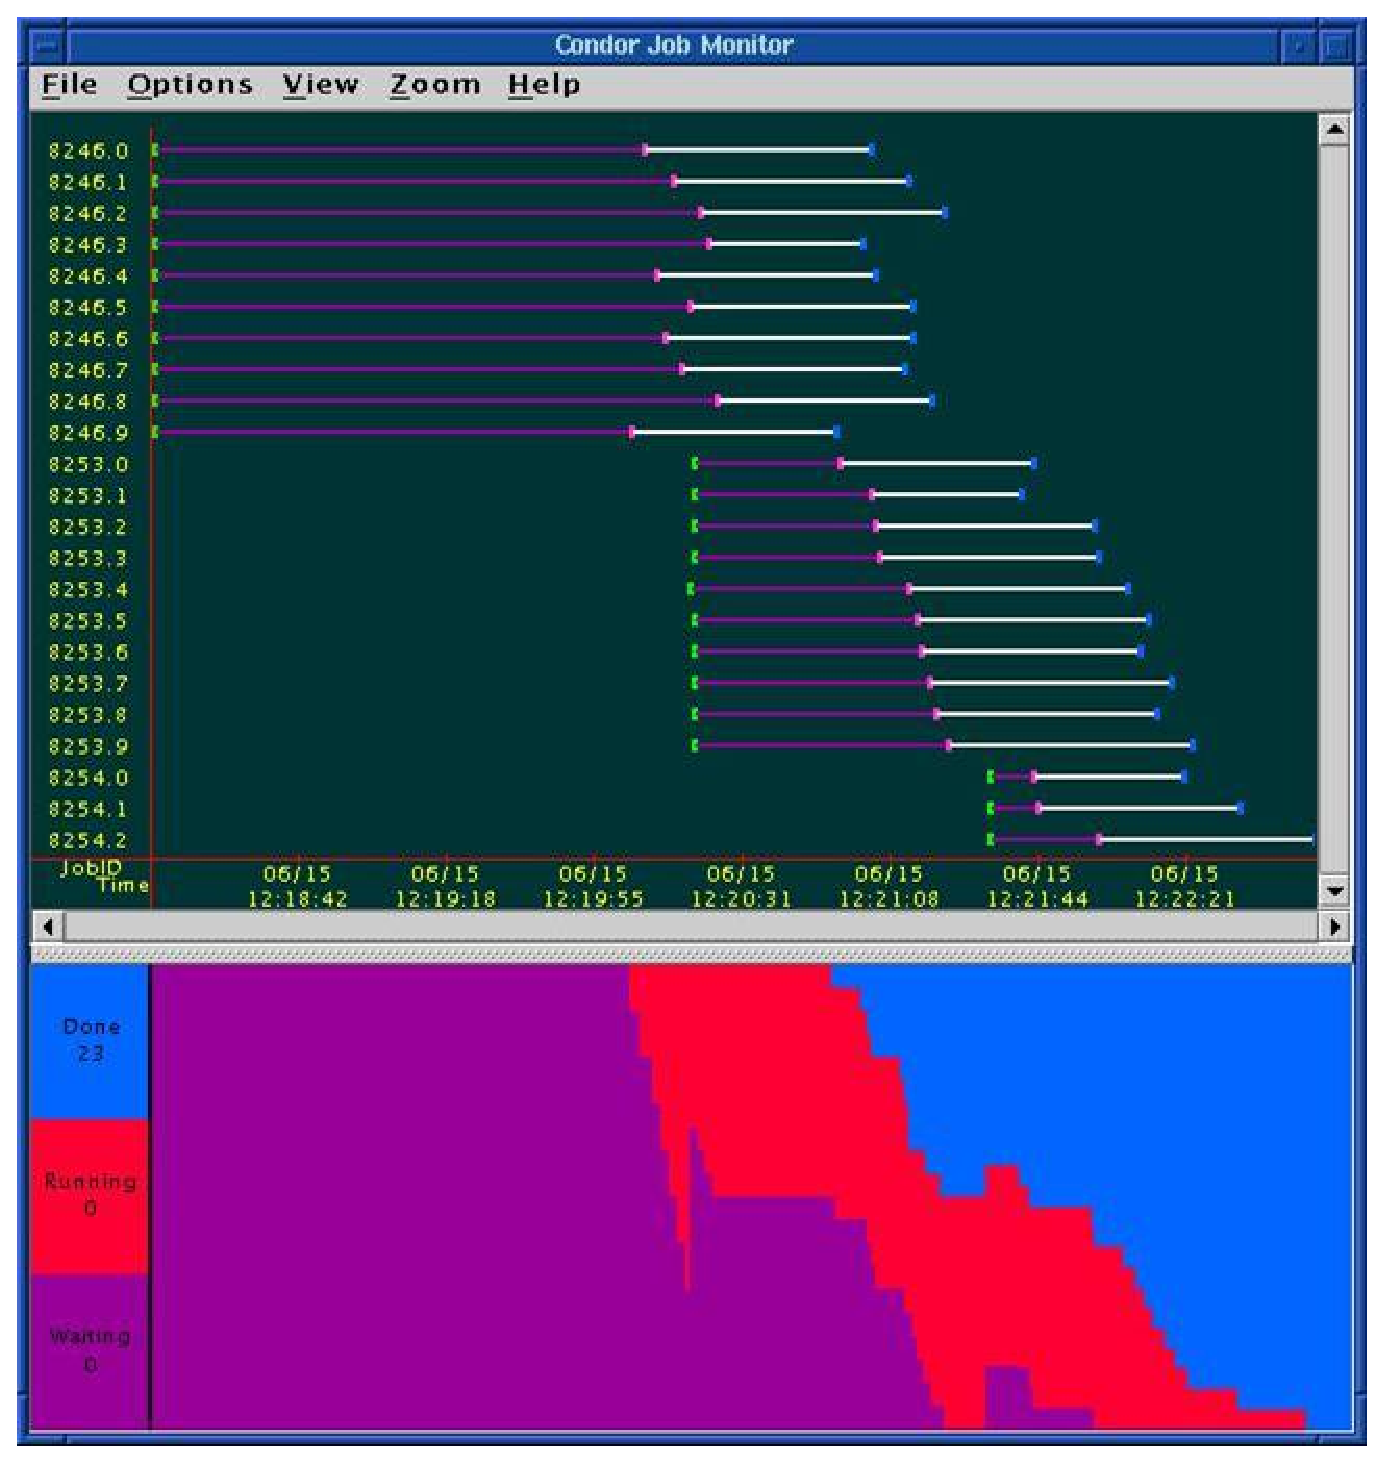
\includegraphics[width=\textwidth]{condor_job_monitor.ps}
    \caption{Condor Job Monitor}
    \label{fig:job_monitor}
  \end{center}
\end{figure}


\subsection{Removing a job from the queue}

A job can be removed from the queue at any time by using the condor\_rm
command. If the job that is being removed is currently running, the job is
killed without a checkpoint, and its queue entry is removed. 

\subsection{Changing the priority of jobs}

In addition to the priorities assigned to each user, Condor also provides each
user with the capability of assigning priorities to each submitted job. These
job priorities are local to each queue and range from -20 to +20, with higher
values meaning better priority.

The default priority of a job is 0, but can be changed using the condor\_prio
command. For example, to change the priority of a job to -15,

\begin{verbatim}
%  condor_q raman

-- Submitter: froth.cs.wisc.edu : <128.105.73.44:33847> : froth.cs.wisc.edu
 ID      OWNER            SUBMITTED    CPU_USAGE ST PRI SIZE CMD               
 126.0   raman           4/11 15:06   0+00:00:00 I  0   0.3  hello             

1 jobs; 1 idle, 0 running, 0 held

%  condor_prio -p -15 126.0

%  condor_q raman

-- Submitter: froth.cs.wisc.edu : <128.105.73.44:33847> : froth.cs.wisc.edu
 ID      OWNER            SUBMITTED    CPU_USAGE ST PRI SIZE CMD               
 126.0   raman           4/11 15:06   0+00:00:00 I  -15 0.3  hello             

1 jobs; 1 idle, 0 running, 0 held
\end{verbatim}

It is important to note that these job priorities are completely different from
the user priorities assigned by Condor. Job priorities do not impact user
priorities. They are only a mechanism for the user to identify the relative
importance of jobs among all the jobs submitted by the user to that specific
queue.


\subsection{Why does the job not run?}

Users sometimes find that their jobs do not run. There are several reasons why a
specific job does not run. These reasons include failed job or machine
constraints, bias due to preferences, insufficient priority, etc. Many of these
reasons can be diagnosed by using the -analyze option of condor\_q. 

\begin{verbatim}
[adrians@trevina ~]$ condor_submit myjob.submit 
Submitting job(s).
Logging submit event(s).
1 job(s) submitted to cluster 1.

[adrians@trevina ~]$ condor_q -analyze


-- Submitter: trevina.iac.es : <161.72.81.178:39869> : trevina.iac.es
 ID      OWNER            SUBMITTED     RUN_TIME ST PRI SIZE CMD               
---
001.000:  Run analysis summary.  Of 187 machines,
    187 are rejected by your job's requirements
      0 reject your job because of their own requirements
      0 match, but are serving users with a better priority in the pool
      0 match, but prefer another specific job despite its worse user-priority
      0 match, but will not currently preempt their existing job
      0 are available to run your job
        No successful match recorded.
        Last failed match: Thu Sep 16 12:38:09 2004
        Reason for last match failure: no match found

WARNING:  Be advised:
   No resources matched request's constraints
   Check the Requirements expression below:

Requirements = ((Memory > 2147483647)) && (Arch == "INTEL") &&
(OpSys == "LINUX") && (Disk >= DiskUsage) &&
(TARGET.FileSystemDomain == MY.FileSystemDomain)
\end{verbatim}

In this example we can see that the job 1.0 has problems to run: its
requirements are too demanding on RAM, and there are no machines that can cope
with this job.

While the analyzer can diagnose most common problems, there are some situations
that it cannot reliably detect due to the instantaneous and local nature of the
information it uses to detect the problem. Thus, it may be that the analyzer
reports that resources are available to service the request, but the job still
does not run. In most of these situations, the delay is transient, and the job
will run during the next negotiation cycle.

If the problem persists and the analyzer is unable to detect the situation, it
may be that the job begins to run but immediately terminates due to some
problem. Viewing the job's error and log files (specified in the submit command
file) may assist in tracking down the problem. If the cause is still unclear,
please contact your system administrator.


\subsection{Job Completion}

When your Condor job completes (either through normal means or abnormal
termination by signal), Condor will remove it from the job queue (i.e., it will
no longer appear in the output of condor\_q) and insert it into the job history
file. You can examine the job history file with the condor\_history command. If
you specified a log file in your submit description file, then the job exit
status will be recorded there as well.

By default, Condor will send you an email message when your job completes. You
can modify this behavior with the condor\_submit ``notification'' command. The
message will include the exit status of your job (i.e., the argument your job
passed to the exit system call when it completed) or notification that your job
was killed by a signal. 


\subsection{Exercise}
\label{ex_condor_history}

Use the condor\_history command to find all the jobs belonging to the user
``adrians'' that were removed from the queue before completing. The history of
submitted jobs is different for each machine, so for this you will have to be
connected to guinda.

To get this right you should probably look at

\htmladdnormallink{http://goya/inves/SINFIN/Condor/v6.6/4\_1Condor\_s\_ClassAd.html}{http://goya/inves/SINFIN/Condor/v6.6/4\_1Condor\_s\_ClassAd.html}



\section{Standard Universe}
In the standard universe, Condor provides checkpointing and remote system
calls. These features make a job more reliable and allow it uniform access to
resources from anywhere in the pool. To prepare a program as a standard universe
job, it must be relinked with condor\_compile. Most programs can be prepared as
a standard universe job, but there are a few restrictions.

Condor checkpoints a job at regular intervals. A checkpoint image is essentially
a snapshot of the current state of a job. If a job must be migrated from one
machine to another, Condor makes a checkpoint image, copies the image to the new
machine, and restarts the job continuing the job from where it left off. If a
machine should crash or fail while it is running a job, Condor can restart the
job on a new machine using the most recent checkpoint image. In this way, jobs
can run for months or years even in the face of occasional computer failures.

To convert your program into a standard universe job, you must use condor\_
compile to relink it with the Condor libraries. Put condor\_compile in front of
your usual link command. You do not need to modify the program's source code,
but you do need access to the unlinked object files. A commercial program that
is packaged as a single executable file cannot be converted into a standard
universe job.

For example, if you would have linked the job by executing:

\begin{verbatim}
% cc main.o tools.o -o program
\end{verbatim}

Then, relink the job for Condor with:

\begin{verbatim}
% condor_compile cc main.o tools.o -o program
\end{verbatim}

There are a few restrictions on standard universe jobs. Before you plan to run a
standard universe job, you should make sure that you check out these restrictions
 in section 2.4.1.1 of the manual page

http://goya/inves/SINFIN/Condor/v6.6/2\_4Road\_map\_Running.html.


At the IAC, we have opted to only do a partial install of
condor\_compile. Because of this you are restricted to using condor\_compile
with one of these programs:

\begin{itemize}
\item cc (the system C compiler) 
\item acc (ANSI C compiler, on Sun systems) 
\item c89 (POSIX compliant C compiler, on some systems) 
\item CC (the system C++ compiler) 
\item f77 (the system FORTRAN compiler) 
\item gcc (the GNU C compiler) 
\item g++ (the GNU C++ compiler) 
\item g77 (the GNU FORTRAN compiler) 
\item ld (the system linker)  
\item f90 (the system FORTRAN 90 compiler), only supported on Solaris and Digital Unix. 
\end{itemize}


\subsubsection{Example}
\paragraph{Our very useful program!}

This program will just loop. In a fast machine it should take about three hours
to finish.

\begin{verbatim}
#include <stdio.h>

int main (int argc, char *argv[])
{
  long this_number, other_number;

this_number = 1;

 while(this_number < 10000000) {
   other_number = 1;

   while(other_number < 100000) {
   if (!(this_number % 1000) && (other_number == 1))
     printf("%ld\n", this_number);
   other_number = other_number + 1;
   }
   this_number = this_number + 1;
 }
 return 0;
}
\end{verbatim}

\paragraph{Submission file}
\begin{verbatim}
########################################################
##
## Example Standard Universe
##
## File: submit_looping_std
##
########################################################

executable = looping_std_solaris_stripped
universe = standard
Requirements = Arch == "SUN4u" && OpSys == "SOLARIS29"

Initialdir = /net/guinda/scratch/angelv/Condor-Course/
output = std_universe.out
error =  std_universe.err
log =    std_universe.log
queue 
\end{verbatim}

\paragraph{Running the code}

\begin{verbatim}
naranja(97)~/SCRIPTS/CONDOR/> condor_compile cc -o looping_std_solaris looping.c 
LINKING FOR CONDOR : /usr/ccs/bin/ld
/opt/SUNWspro/SC5.0/lib/crti.o /usr/pkg/condor/condor-6.6.3/lib/condor_rt0.o
/opt/SUNWspro/SC5.0/lib/values-xa.o -o looping_std_solaris looping.o -Y
P,/opt/SUNWspro/SC5.0/lib:/usr/ccs/lib: /usr/lib -Qy
/usr/pkg/condor/condor-6.6.3/lib/libcondorzsyscall.a
/usr/pkg/condor/condor-6.6.3/lib/libz.a -Bdynamic -lsocket -lnsl -lc
/opt/SUNWspro/SC5.0/lib/crtn.o
/usr/pkg/condor/condor-6.6.3/lib/libcondorc++support.a


naranja(102)~/SCRIPTS/CONDOR/> cp looping_std_solaris looping_std_solaris_stripped

naranja(103)~/SCRIPTS/CONDOR/> strip looping_std_solaris_stripped

naranja(107)~/SCRIPTS/CONDOR/> ls -l
total 41728
-rwxr-xr-x   1 angelv   other       4673 Sep 29 17:48 looping
-rw-r--r--   1 angelv   other        382 Sep 29 17:47 looping.c
-rwxr-xr-x   1 angelv   other    12327189 Sep 29 17:53 looping_std_linux
-rwxr-xr-x   1 angelv   other    1333784 Sep 29 17:56 looping_std_linux_stripped
-rwxr-xr-x   1 angelv   other    5678624 Sep 29 17:54 looping_std_solaris
-rwxr-xr-x   1 angelv   other     678676 Sep 29 17:55 looping_std_solaris_stripped
-rw-r--r--   1 angelv   other        138 May 26 16:52 submit_looping_std
naranja(108)~/SCRIPTS/CONDOR/>

naranja(106)~/SCRIPTS/CONDOR/> ./looping_std_solaris_stripped
Condor: Notice: Will checkpoint to ./looping_std_solaris_stripped.ckpt
Condor: Notice: Remote system calls disabled.
1000
2000
[...]
naranja(107)~/SCRIPTS/CONDOR/>

-------------------------------------------------------------------------

naranja(107)~/SCRIPTS/CONDOR/> cat /scratch/angelv/Condor-Course/std_universe.log

000 (188.000.000) 09/29 18:24:30 Job submitted from host: <161.72.81.187:51962>
...
001 (188.000.000) 09/29 18:25:16 Job executing on host: <161.72.65.35:37169>
...
006 (188.000.000) 09/29 18:27:22 Image size of job updated: 2961
...
004 (188.000.000) 09/29 18:27:30 Job was evicted.
	(1) Job was checkpointed.
		Usr 0 00:02:03, Sys 0 00:00:00  -  Run Remote Usage
		Usr 0 00:00:00, Sys 0 00:00:00  -  Run Local Usage
	2353744  -  Run Bytes Sent By Job
	680030  -  Run Bytes Received By Job
...
001 (188.000.000) 09/29 18:31:21 Job executing on host: <161.72.65.35:37169>
...
004 (188.000.000) 09/29 18:33:31 Job was evicted.
	(1) Job was checkpointed.
		Usr 0 00:01:56, Sys 0 00:00:00  -  Run Remote Usage
		Usr 0 00:00:00, Sys 0 00:00:00  -  Run Local Usage
	2353400  -  Run Bytes Sent By Job
	3032210  -  Run Bytes Received By Job
...
001 (188.000.000) 09/29 18:42:26 Job executing on host: <161.72.65.11:44853>
...
004 (188.000.000) 09/29 20:05:02 Job was evicted.
	(1) Job was checkpointed.
		Usr 0 01:20:57, Sys 0 00:00:00  -  Run Remote Usage
		Usr 0 00:00:00, Sys 0 00:00:00  -  Run Local Usage
	2353400  -  Run Bytes Sent By Job
	3032146  -  Run Bytes Received By Job
...
001 (188.000.000) 09/29 20:13:26 Job executing on host: <161.72.69.18:45267>
...
006 (188.000.000) 09/30 02:13:41 Image size of job updated: 2993
...
003 (188.000.000) 09/30 02:14:19 Job was checkpointed.
	Usr 0 05:57:16, Sys 0 00:00:00  -  Run Remote Usage
		Usr 0 00:00:00, Sys 0 00:00:00  -  Run Local Usage
...
003 (188.000.000) 09/30 08:14:11 Job was checkpointed.
	Usr 0 11:53:43, Sys 0 00:00:00  -  Run Remote Usage
		Usr 0 00:00:00, Sys 0 00:00:00  -  Run Local Usage
...

[...]

...
001 (188.000.000) 09/30 11:58:17 Job executing on host: <161.72.66.25:61440>
...


[angelv@guinda Condor-Course]$ condor_q

-- Submitter: guinda.iac.es : <161.72.81.187:51962> : guinda.iac.es
 ID      OWNER            SUBMITTED     RUN_TIME ST PRI SIZE CMD
 188.0   angelv          9/29 18:24   0+18:26:51 R  0   2.9  looping_std_solari

1 jobs; 0 idle, 1 running, 0 held


[angelv@guinda Condor-Course]$ condor_q -l 188.0
-- Submitter: guinda.iac.es : <161.72.81.187:51962> : guinda.iac.es
MyType = "Job"
TargetType = "Machine"
ClusterId = 188
QDate = 1096478669
[...]
Iwd = "/net/guinda/scratch/angelv/Condor-Course/"
JobUniverse = 1
Cmd = "/home/angelv/Condor-Course/Standard_Universe/looping_std_solaris_stripped"
[...]
Requirements = (Arch == "SUN4u" && OpSys == "SOLARIS29") && 
               ((CkptArch == Arch) || (CkptArch =?= UNDEFINED)) && 
               ((CkptOpSys == OpSys) || (CkptOpSys =?= UNDEFINED)) && 
               (Disk >= DiskUsage) && ((Memory * 1024) >= ImageSize)
[...]
TotalSuspensions = 6
CumulativeSuspensionTime = 2853
[...]
NumCkpts = 8
NumRestarts = 13
CkptArch = "SUN4u"
CkptOpSys = "SOLARIS29"
RemoteWallClockTime = 61103.000000
LastRemoteHost = "avestruz.ll.iac.es"
[...]
RemoteHost = "gata.ll.iac.es"
RemoteVirtualMachineID = 1
ShadowBday = 1096541885
JobLastStartDate = 1096539606
JobCurrentStartDate = 1096541885
JobRunCount = 7
WallClockCheckpoint = 4242
ServerTime = 1096547198

[angelv@guinda Condor-Course]$

\end{verbatim}

\section{DAGMan}

A directed acyclic graph (DAG) can be used to represent a set of programs where
the input, output, or execution of one or more programs is dependent on one or
more other programs. The programs are nodes (vertices) in the graph, and the
edges (arcs) identify the dependencies. Condor finds machines for the execution
of programs, but it does not schedule programs (jobs) based on dependencies. The
Directed Acyclic Graph Manager (DAGMan) is a meta-scheduler for Condor
jobs. DAGMan submits jobs to Condor in an order represented by a DAG and
processes the results. An input file defined prior to submission describes the
DAG, and a Condor submit description file for each program in the DAG is used by
Condor.

Each node (program) in the DAG specifies a Condor submit description file. As
DAGMan submits jobs to Condor, it monitors the Condor log file(s) to enforce the
ordering required for the DAG. The DAG itself is defined by the contents of a
DAGMan input file. DAGMan is responsible for scheduling, recovery, and reporting
for the set of programs submitted to Condor.

One limitation exists: each Condor submit description file must submit only one
job. There may not be multiple queue commands, or DAGMan will fail. This
requirement exists to enforce the requirements of a well-defined DAG. If each
node of the DAG could cause the submission of multiple Condor jobs, then it
would violate the definition of a DAG.

DAGMan no longer requires that all jobs specify the same log file. However, if
the DAG contains a very large number of jobs, each specifying its own log file,
performance may suffer. Therefore, if the DAG contains a large number of jobs,
it is best to have all of the jobs use the same log file. DAGMan enforces the
dependencies within a DAG using the events recorded in the log file(s) produced
by job submission to Condor.


\subsection{Basic DAGs} 

\subsubsection{Example}
\paragraph{Submission file}

\begin{verbatim}
# Filename: diamond.dag
#
Job  A  A.condor 
Job  B  B.condor 
Job  C  C.condor	
Job  D  D.condor
PARENT A CHILD B C
PARENT B C CHILD D

--------------------------------------------

########################################################
##
## A.condor
##
## Simple condor job description file
##
########################################################

executable = basic.sh
universe = vanilla
output = A.out
error =  A.err
log =    dagman_example.log
queue

----------------------------------------

#!/bin/sh

# Filename: basic.sh
#

echo Executed on `uname -n` at `date`
\end{verbatim}

\paragraph{Running the code}
\begin{verbatim}
naranja(27)~/Condor-Course/dagman1> condor_submit_dag diamond.dag

Checking your DAG input file and all submit files it references.
This might take a while...
Done.
-----------------------------------------------------------------------
File for submitting this DAG to Condor           : diamond.dag.condor.sub
Log of DAGMan debugging messages                 : diamond.dag.dagman.out
Log of Condor library debug messages             : diamond.dag.lib.out
Log of the life of condor_dagman itself          : diamond.dag.dagman.log

Condor Log file for all Condor jobs of this DAG: dagman_example.log
Submitting job(s).
Logging submit event(s).
1 job(s) submitted to cluster 3548.
-----------------------------------------------------------------------
naranja(28)~/Condor-Course/dagman1>


naranja(63)~/Condor-Course/dagman1> condor_q -dag angelv


-- Submitter: naranja.iac.es : <161.72.64.97:49674> : naranja.iac.es
 ID      OWNER/NODENAME   SUBMITTED     RUN_TIME ST PRI SIZE CMD
3548.0   angelv          9/28 09:55   0+00:00:11 R  0   4.0  condor_dagman -f -
3549.0    |-A            9/28 09:55   0+00:00:00 I  0   0.0  basic.sh

2 jobs; 1 idle, 1 running, 0 held
naranja(64)~/Condor-Course/dagman1>



naranja(40)~/Condor-Course/dagman1> condor_q angelv


-- Submitter: naranja.iac.es : <161.72.64.97:49674> : naranja.iac.es
 ID      OWNER            SUBMITTED     RUN_TIME ST PRI SIZE CMD

0 jobs; 0 idle, 0 running, 0 held
naranja(41)~/Condor-Course/dagman1>


naranja(43)~/Condor-Course/dagman1> cat A.out
Executed on albatros at Tue Sep 28 10:00:45 WEST 2004
naranja(44)~/Condor-Course/dagman1> cat B.out
Executed on albatros at Tue Sep 28 10:01:51 WEST 2004
naranja(45)~/Condor-Course/dagman1> cat C.out
Executed on asno at Tue Sep 28 10:01:51 WEST 2004
naranja(46)~/Condor-Course/dagman1> cat D.out
Executed on albatros at Tue Sep 28 10:02:35 WEST 2004
naranja(47)~/Condor-Course/dagman1>
\end{verbatim}

\subsubsection{Exercise}
\label{ex_basic_dag}
In the previous example, all the jobs could actually run in parallel, since no
job depends on the output of any other. Your task for this exercise is to modify
the jobs, the submission files, etc. as follows: job A should create two files,
B.input and C.input containing a line of text. Job B reads B.input and generates
B.output where the text in B.input is modified in any way you want. Likewise for
job C. Job D should take the text in B.output and C.output and print to standard
output the contents of both files. Run it and verify that all is working
according to plan.


\subsection{Let's go for the real thing\dots}

\subsubsection{DAGs with PRE and POST processing}

In a DAGMan you can also specify processing that is done either before a program
within the DAG is submitted to Condor for execution or after a program within
the DAG completes its execution. Processing done before a program is submitted
to Condor is called a PRE script. Processing done after a program successfully
completes its execution under Condor is called a POST script. A node in the DAG
is comprised of the program together with PRE and/or POST scripts. The
dependencies in the DAG are enforced based on nodes.

DAGMan takes note of the exit value of the scripts as well as the program. If
the PRE script fails (exit value != 0), then neither the program nor the POST
script runs, and the node is marked as failed.

If the PRE script succeeds, the program is submitted to Condor. If the program
fails and there is no POST script, the DAG node is marked as failed. An exit
value not equal to 0 indicates program failure. It is therefore important that
the program returns the exit value 0 to indicate the program did not fail.

If the program fails and there is a POST script, node failure is determined by
the exit value of the POST script. A failing value from the POST script marks
the node as failed. A succeeding value from the POST script (even with a failed
program) marks the node as successful. Therefore, the POST script may need to
consider the return value from the program.

By default, the POST script is run regardless of the program's return value. To
prevent POST scripts from running after failed jobs, pass the -NoPostFail
argument to condor\_ submit\_dag.

A node not marked as failed at any point is successful.

Two variables are available to ease script writing. The \$JOB variable evaluates
to JobName. For POST scripts, the \$RETURN variable evaluates to the return value
of the program. The variables may be placed anywhere within the arguments.

\subsubsection{Job recovery: the rescue DAG}

DAGMan can help with the resubmission of uncompleted portions of a DAG when one
or more nodes resulted in failure. If any node in the DAG fails, the remainder
of the DAG is continued until no more forward progress can be made based on the
DAG's dependencies. At this point, DAGMan produces a file called a Rescue DAG.

The Rescue DAG is a DAG input file, functionally the same as the original DAG
file. It additionally contains indication of successfully completed nodes using
the DONE option in the input description file. If the DAG is resubmitted using
this Rescue DAG input file, the nodes marked as completed will not be
re-executed.

\subsubsection{Macros in DAG files}

In a DAG input file there is a method for defining a macro to be placed into the
submit description files. It can be used to dramatically reduce the number of
submit description files needed for a DAG. In the case where the submit
description file for each node varies only in file naming, the use of a
substitution macro within the submit description file allows the use of a single
submit description file. Note that the node output log file currently cannot be
specified using a macro passed from the DAG.

The example uses a single submit description file in the DAG input file, and
uses the Vars entry to name output files.

\begin{verbatim}
# submit description file called:  theonefile.sub
executable   = progX
output       = \$(outfilename)
error        = error.\$(outfilename)
universe     = standard
queue
\end{verbatim}

The relevant portion of the DAG input file appears as

\begin{verbatim}
JOB A theonefile.sub
JOB B theonefile.sub
JOB C theonefile.sub

VARS A outfilename="A"
VARS B outfilename="B"
VARS C outfilename="C"
\end{verbatim}

For a DAG like this one with thousands of nodes, being able to write and
maintain a single submit description file and a single, yet more complex, DAG
input file is preferable.

\subsection{Exercises}
\label{ex_advanced_dag}
For this exercise we are going to modify the files created for the exercise
given in section \ref{ex_basic_dag} as follows. 

\begin{enumerate}
\item In the previous exercise a lot of files were created, some of which were
only temporary ones. We will use the POST arguments to make use of
scripts that will delete these temporary files, and also create a script that
will compress the final output file.

\item Once you have it working, write a PRE script for the node C so that it will
  fail. Try to run it and see how a rescue file is created. Edit the created
  rescue file, so that we don't invoke again the PRE script. Resubmit using the
  rescue DAG file and see what happens...
\end{enumerate}


\section{Last remarks}
While we have covered most of what you would normally use with Condor, there are
also some other functionalities worth exploring:

\begin{itemize}
\item The Java Universe, which is better suited to run Java applications. More
  info at http://www.cs.wisc.edu/condor/manual/v6.6/2\_8Java\_Applications.html
\item The possibility of creating DAGs within DAGs for really complex job
  dependencies. See section 2.11.9 in 

http://goya/inves/SINFIN/Condor/v6.6/2\_11DAGMan\_Applications.html
\item If you need more power for your job dependencies, you can use the Perl
  module described in

  http://www.cs.wisc.edu/condor/manual/v6.6/4\_4Condor\_Perl.html. With it you
  can create very versatile dependencies, including conditional branches, cycles, etc.
\end{itemize}

Condor is a project in constant development and many other interesting research
areas are being pursued. If you would like to find out about all this, check
its official webpage at \htmladdnormallink{http://www.cs.wisc.edu/condor/}{http://www.cs.wisc.edu/condor/}

Enjoy Condor!

\newpage
\appendix

\section{Answers to exercises}

\subsection{Answers to exercises in section \ref{ex_condor_status}}

\begin{enumerate}
\item \begin{verbatim}condor_status -constraint OpSys==\"LINUX\" -sort Memory\end{verbatim}
\item \begin{verbatim}
condor_status -java -constraint 'OpSys == "SOLARIS29"'
 -format "The machine %s " Machine -format "has Java Version: %s \n" JavaVersion
\end{verbatim}
\end{enumerate}


\subsection{Answer to exercise in section \ref{ex_disk_info}}

The disk\_info.sh file could be:

\begin{verbatim}
#!/bin/sh
echo `uname -n`
df -h | grep " /scratch"
\end{verbatim}

Given this file, a basic submission file for it would be:

\begin{verbatim}
########################################################
##
## Sample solution for exercise 1
##
##
########################################################

executable = disk_info.sh
universe = vanilla
output = exercise1.out
error =  exercise1.err
log =    exercise1.log
queue
\end{verbatim}

\subsection{Answer to exercise in section \ref{ex_R}}

After you have created test0.R and test1.R to contain the different instructions
to R, you could submit to Condor the following file:

\begin{verbatim}
########################################################
##
## Exercise 2
##
## A realistic submission file
##
########################################################

executable = /usr/local/bin/R
universe = vanilla
Requirements = Memory >= 1000 && ((Arch == "INTEL" && OpSys == "LINUX") || \
                                  (Arch == "SUN4u" && OpSys == "SOLARIS29"))
Rank = Memory

Initialdir = /net/guinda/scratch/angelv/Condor-Course/
arguments = --vanilla
input = test$(Process).R
output = exercise2.$(Process).out
error =  exercise2.$(Process).err
log =    exercise2.log
queue 2
\end{verbatim}

\subsection{Answer to exercise in section \ref{ex_condor_history}}

\begin{verbatim}
[angelv@guinda ~/Condor-Course]$ condor_history -constraint 
                            'RemoveReason=!=UNDEFINED && User=="adrians@iac.es"'
(RemoveReason=!=UNDEFINED && User=="adrians@iac.es")
 ID      OWNER            SUBMITTED     RUN_TIME ST   COMPLETED CMD
 143.0   adrians         7/27 11:51   0+00:00:23 X   ???        /home/adrians/c
 144.0   adrians         7/27 11:52   0+00:00:52 X   ???        /home/adrians/c
 144.4   adrians         7/27 11:52   0+00:00:51 X   ???        /home/adrians/c
 144.5   adrians         7/27 11:52   0+00:00:49 X   ???        /home/adrians/c
 144.8   adrians         7/27 11:52   0+00:00:57 X   ???        /home/adrians/c
 144.9   adrians         7/27 11:52   0+00:00:55 X   ???        /home/adrians/c
 144.1   adrians         7/27 11:52   0+00:01:03 X   ???        /home/adrians/c
 144.2   adrians         7/27 11:52   0+00:01:01 X   ???        /home/adrians/c
 144.3   adrians         7/27 11:52   0+00:00:59 X   ???        /home/adrians/c
 144.6   adrians         7/27 11:52   0+00:00:50 X   ???        /home/adrians/c
 144.7   adrians         7/27 11:52   0+00:00:48 X   ???        /home/adrians/c
 146.0   adrians         7/27 12:05   0+00:00:12 X   ???        /tmp/adrians/my
 146.1   adrians         7/27 12:05   0+00:00:13 X   ???        /tmp/adrians/my
 146.3   adrians         7/27 12:05   0+00:00:10 X   ???        /tmp/adrians/my
 146.4   adrians         7/27 12:05   0+00:00:10 X   ???        /tmp/adrians/my
 146.2   adrians         7/27 12:05   0+00:00:36 X   ???        /tmp/adrians/my
 147.0   adrians         7/27 12:40   0+06:56:21 X   ???        /tmp/adrians/my
 147.1   adrians         7/27 12:40   0+04:26:55 X   ???        /tmp/adrians/my
 147.2   adrians         7/27 12:40   0+05:14:00 X   ???        /tmp/adrians/my
 147.3   adrians         7/27 12:40   0+04:17:06 X   ???        /tmp/adrians/my
 147.4   adrians         7/27 12:40   0+03:51:35 X   ???        /tmp/adrians/my
[angelv@guinda ~/Condor-Course]$
\end{verbatim}

\subsection{Answer to exercise in section \ref{ex_basic_dag}}

\begin{verbatim}
# Filename: diamond.dag
#
Job  A  A.condor 
Job  B  B.condor 
Job  C  C.condor	
Job  D  D.condor
PARENT A CHILD B C
PARENT B C CHILD D

-----------------------------------------

########################################################
##
## A.condor
##
## Simple condor job description file
##
########################################################
executable = A.sh
universe = vanilla
output = A.out
error =  A.err
log =    dagman_example.log
queue

----------------------------------------

#!/bin/sh
# Filename: A.sh
#
echo This is the output of Job A for Job B > B.input
echo This is the output of Job A for Job C > C.input

----------------------------------------

########################################################
##
## B.condor
##
## Simple condor job description file
##
########################################################
executable = B.sh
universe = vanilla
output = B.out
error =  B.err
log =    dagman_example.log
queue

----------------------------------------

#!/bin/sh
# Filename: B.sh
#
echo `cat B.input` after being massaged by Job B >> B.output

----------------------------------------

########################################################
##
## C.condor
##
## Simple condor job description file
##
########################################################
executable = C.sh
universe = vanilla
output = C.out
error =  C.err
log =    dagman_example.log
queue

----------------------------------------

#!/bin/sh
# Filename: C.sh
#
echo `cat C.input` after being massaged by Job C >> C.output

----------------------------------------

########################################################
##
## D.condor
##
## Simple condor job description file
##
########################################################
executable = D.sh
universe = vanilla
output = D.out
error =  D.err
log =    dagman_example.log
queue

----------------------------------------

#!/bin/sh
# Filename: D.sh
#
cat B.output C.output
\end{verbatim}

After running the code, your directory should look like:

\begin{verbatim}
  /home/angelv/Condor-Course/Exercises/dagman1:
  used 26 available 50764572
  -rw-r--r--    1 angelv   games         275 sep 30 14:17 A.condor
  -rw-r--r--    1 angelv   games           0 sep 30 14:19 A.err
  -rw-r--r--    1 angelv   games           0 sep 30 14:19 A.out
  -rwxr-xr-x    1 angelv   games         138 sep 30 14:08 A.sh
  -rw-r--r--    1 angelv   games         275 sep 30 14:17 B.condor
  -rw-r--r--    1 angelv   games           0 sep 30 14:20 B.err
  -rw-r--r--    1 angelv   games          38 sep 30 14:19 B.input
  -rw-r--r--    1 angelv   games           0 sep 30 14:20 B.out
  -rw-r--r--    1 angelv   games          68 sep 30 14:20 B.output
  -rwxr-xr-x    1 angelv   games          93 sep 30 14:11 B.sh
  -rw-r--r--    1 angelv   games         275 sep 30 14:17 C.condor
  -rw-r--r--    1 angelv   games           0 sep 30 14:20 C.err
  -rw-r--r--    1 angelv   games          38 sep 30 14:19 C.input
  -rw-r--r--    1 angelv   games           0 sep 30 14:20 C.out
  -rw-r--r--    1 angelv   games          68 sep 30 14:20 C.output
  -rwxr-xr-x    1 angelv   games          93 sep 30 14:12 C.sh
  -rw-------    1 angelv   games        2486 sep 30 14:21 dagman_example.log
  -rw-r--r--    1 angelv   games         275 sep 30 14:17 D.condor
  -rw-r--r--    1 angelv   games           0 sep 30 14:21 D.err
  -rw-r--r--    1 angelv   games         135 sep 28 09:46 diamond.dag
  -rw-r--r--    1 angelv   games         508 sep 30 14:17 diamond.dag.condor.sub
  -rw-r--r--    1 angelv   games         606 sep 30 14:21 diamond.dag.dagman.log
  -rw-r--r--    1 angelv   games        5516 sep 30 14:21 diamond.dag.dagman.out
  -rw-r--r--    1 angelv   games          29 sep 30 14:21 diamond.dag.lib.out
  -rw-r--r--    1 angelv   games         136 sep 30 14:21 D.out
  -rwxr-xr-x    1 angelv   games          54 sep 30 14:12 D.sh
\end{verbatim}

You can get the details of everything that happened in the files
dagman\_example\_log and diamond.dag.dagman.out. The important bit, the results,
are in the file D.out and should look like:

\begin{verbatim}
This is the output of Job A for Job B after being massaged by Job B
This is the output of Job A for Job C after being massaged by Job C
\end{verbatim}

\subsection{Answer to exercises in section \ref{ex_advanced_dag}}

\subsubsection{Exercise 1}

You don't need to make many changes for this. One possible solution implies just
changing the diadmon.dag file to:

\begin{verbatim}
# Filename: diamond.dag
#
Job  A  A.condor 
Job  B  B.condor 
Job  C  C.condor	
Job  D  D.condor
SCRIPT POST B post.pl $JOB
SCRIPT POST C post.pl $JOB
SCRIPT POST D post.pl $JOB
PARENT A CHILD B C
PARENT B C CHILD D
\end{verbatim}

And writing a script to take care of the file deletes and compressions. An
example in perl could be:

\begin{verbatim}
#!/usr/bin/perl

# Filename: post.pl
#
if (@ARGV[0] eq "B") {
    unlink "B.input";
} elsif (@ARGV[0] eq "C") {
    unlink "C.input";
} elsif (@ARGV[0] eq "D") {
    unlink "B.output";
    unlink "C.output";
    system "gzip D.out";
}
\end{verbatim}


With these changes, when we submit the job to condor, we end up without
temporary files, and with a gzipped results file (of course we could also
automatically delete all the *.err and *.out files, etc.):

\begin{verbatim}
  /home/angelv/Condor-Course/Exercises/dagman_advanced_1:
  used 24 available 50671203
  -rw-r--r--    1 angelv   games         275 sep 30 14:17 A.condor
  -rw-r--r--    1 angelv   games           0 sep 30 15:49 A.err
  -rw-r--r--    1 angelv   games           0 sep 30 15:49 A.out
  -rwxr-xr-x    1 angelv   games         138 sep 30 14:08 A.sh
  -rw-r--r--    1 angelv   games         275 sep 30 14:17 B.condor
  -rw-r--r--    1 angelv   games           0 sep 30 15:50 B.err
  -rw-r--r--    1 angelv   games           0 sep 30 15:50 B.out
  -rwxr-xr-x    1 angelv   games          93 sep 30 14:11 B.sh
  -rw-r--r--    1 angelv   games         275 sep 30 14:17 C.condor
  -rw-r--r--    1 angelv   games           0 sep 30 15:50 C.err
  -rw-r--r--    1 angelv   games           0 sep 30 15:50 C.out
  -rwxr-xr-x    1 angelv   games          93 sep 30 14:12 C.sh
  -rw-------    1 angelv   games        2794 sep 30 15:51 dagman_example.log
  -rw-r--r--    1 angelv   games         275 sep 30 14:17 D.condor
  -rw-r--r--    1 angelv   games           0 sep 30 15:51 D.err
  -rw-r--r--    1 angelv   games         216 sep 30 15:29 diamond.dag
  -rw-r--r--    1 angelv   games         508 sep 30 15:48 diamond.dag.condor.sub
  -rw-r--r--    1 angelv   games         606 sep 30 15:52 diamond.dag.dagman.log
  -rw-r--r--    1 angelv   games        6882 sep 30 15:52 diamond.dag.dagman.out
  -rw-r--r--    1 angelv   games          29 sep 30 15:52 diamond.dag.lib.out
  -rw-r--r--    1 angelv   games          94 sep 30 15:51 D.out.gz
  -rwxr-xr-x    1 angelv   games          54 sep 30 14:12 D.sh
  -rwxr-xr-x    1 angelv   games         214 sep 30 15:46 post.pl
\end{verbatim}

\subsubsection{Exercise 2}

In order to make the node fail, we could change the diamong.dag file to:

\begin{verbatim}
# Filename: diamond.dag
#
Job  A  A.condor 
Job  B  B.condor 
Job  C  C.condor	
Job  D  D.condor

SCRIPT POST B post.pl $JOB
SCRIPT PRE C pre.pl $JOB
SCRIPT POST C post.pl $JOB
SCRIPT POST D post.pl $JOB
PARENT A CHILD B C
PARENT B C CHILD D
\end{verbatim}

So now the script pre.pl will run before job C. Let's make the script pre.pl
fail by writing a syntax error:

\begin{verbatim}
#!/usr/bin/perl

# Filename: pre.pl
#
if (@ARGV[0] eq "C") {
    unlin "C.input";
} 
\end{verbatim}


If we now submit the job, we will find that after a while, the job gets
unqueued, and by looking at the end of file diamond.dag.dagman.out we get:

\begin{verbatim}
[...]
9/30 16:13:19 Job A completed successfully.
9/30 16:13:19 Running PRE script of Job C...
9/30 16:13:19 Of 4 nodes total:
9/30 16:13:19  Done     Pre   Queued    Post   Ready   Un-Ready   Failed
9/30 16:13:19   ===     ===      ===     ===     ===        ===      ===
9/30 16:13:19     1       1        0       0       1          1        0
9/30 16:13:19 PRE Script of Job C failed with status 9
9/30 16:13:25 Submitting Condor Job B ...
9/30 16:13:25 submitting: condor_submit  -a 'dag_node_name = B' -a '+DAGManJobID
         = 224.0' -a 'submit_event_notes = DAG Node: $(dag_node_name)' B.condor 2>&1
9/30 16:13:27 	assigned Condor ID (226.0.0)
9/30 16:13:27 Just submitted 1 job this cycle...
9/30 16:13:27 Event: ULOG_SUBMIT for Condor Job B (226.0.0)
9/30 16:13:27 Of 4 nodes total:
9/30 16:13:27  Done     Pre   Queued    Post   Ready   Un-Ready   Failed
9/30 16:13:27   ===     ===      ===     ===     ===        ===      ===
9/30 16:13:27     1       0        1       0       0          1        1
9/30 16:14:12 Event: ULOG_EXECUTE for Condor Job B (226.0.0)
9/30 16:14:12 Event: ULOG_JOB_TERMINATED for Condor Job B (226.0.0)
9/30 16:14:12 Job B completed successfully.
9/30 16:14:12 Running POST script of Job B...
9/30 16:14:12 Of 4 nodes total:
9/30 16:14:12  Done     Pre   Queued    Post   Ready   Un-Ready   Failed
9/30 16:14:12   ===     ===      ===     ===     ===        ===      ===
9/30 16:14:12     1       0        0       1       0          1        1
9/30 16:14:17 Event: ULOG_POST_SCRIPT_TERMINATED for Condor Job B (226.0.0)
9/30 16:14:17 POST Script of Job B completed successfully.
9/30 16:14:17 Of 4 nodes total:
9/30 16:14:17  Done     Pre   Queued    Post   Ready   Un-Ready   Failed
9/30 16:14:17   ===     ===      ===     ===     ===        ===      ===
9/30 16:14:17     2       0        0       0       0          1        1
9/30 16:14:17 ERROR: the following job(s) failed:
9/30 16:14:17 ---------------------- Job ----------------------
9/30 16:14:17       Node Name: C
9/30 16:14:17          NodeID: 2
9/30 16:14:17     Node Status: STATUS_ERROR    
9/30 16:14:17           Error: PRE Script failed with status 9
9/30 16:14:17 Job Submit File: C.condor
9/30 16:14:17      PRE Script: pre.pl $JOB
9/30 16:14:17     POST Script: post.pl $JOB
9/30 16:14:17   Condor Job ID: [not yet submitted]
9/30 16:14:17       Q_PARENTS: 0, <END>
9/30 16:14:17       Q_WAITING: <END>
9/30 16:14:17      Q_CHILDREN: 3, <END>
9/30 16:14:17 ---------------------------------------	<END>
9/30 16:14:17 Aborting DAG...
9/30 16:14:17 Writing Rescue DAG to diamond.dag.rescue...
9/30 16:14:17 **** condor_scheduniv_exec.224.0 (condor_DAGMAN) EXITING WITH STATUS 1
\end{verbatim}

So, we see that the PRE script of Job C failed, but nevertheless nodes A and B
did complete OK. If we inspect the rescue file created, we see:

\begin{verbatim}
# Rescue DAG file, created after running
#   the diamond.dag DAG file
#
# Total number of Nodes: 4
# Nodes premarked DONE: 2
# Nodes that failed: 1
#   C,<ENDLIST>

JOB A A.condor DONE

JOB B B.condor DONE
SCRIPT POST B post.pl $JOB

JOB C C.condor 
SCRIPT PRE  C pre.pl $JOB
SCRIPT POST C post.pl $JOB

JOB D D.condor 
SCRIPT POST D post.pl $JOB


PARENT A CHILD B C
PARENT B CHILD D
PARENT C CHILD D
\end{verbatim}


This is just a regular DAG submission file, so we can edit it. Note the DONE
tags, which will indicate to Condor not to retry those Jobs. We can just comment
the line for the C PRE script, and submit this DAG rescue file again. As you can
see from the logs, Condor understands that two jobs have already been completed,
and it won't execute them again.

\begin{verbatim}
[angelv@guinda dagman_advanced_2]$ condor_submit_dag diamond.dag.rescue

-----------------------------------------------------------------------
File for submitting this DAG to Condor           : diamond.dag.rescue.condor.sub
Log of DAGMan debugging messages                 : diamond.dag.rescue.dagman.out
Log of Condor library debug messages             : diamond.dag.rescue.lib.out
Log of the life of condor_dagman itself          : diamond.dag.rescue.dagman.log

Condor Log file for all Condor jobs of this DAG: diamond.dag.rescue.dummy_log
Submitting job(s).
Logging submit event(s).
1 job(s) submitted to cluster 401.
-----------------------------------------------------------------------

[angelv@guinda dagman_advanced_2]$ cat diamond.dag.rescue.dagman.out

10/25 10:34:32 ******************************************************
10/25 10:34:32 ** condor_scheduniv_exec.401.0 (CONDOR_DAGMAN) STARTING UP
10/25 10:34:32 ** /home/condor/local.guinda/spool/cluster401.ickpt.subproc0
10/25 10:34:32 ** $CondorVersion: 6.6.7 Oct 11 2004 $
10/25 10:34:32 ** $CondorPlatform: I386-LINUX_RH9 $
10/25 10:34:32 ** PID = 4228
10/25 10:34:32 ******************************************************
10/25 10:34:32 Using config file: /home/condor/condor_config
10/25 10:34:32 Using local config files: /home/condor/condor_config.INTEL.LINUX /home/condor/local.guinda/condor_config.local
10/25 10:34:32 DaemonCore: Command Socket at <161.72.81.187:30023>
10/25 10:34:32 argv[0] == "condor_scheduniv_exec.401.0"
10/25 10:34:32 argv[1] == "-Debug"
10/25 10:34:32 argv[2] == "3"
10/25 10:34:32 argv[3] == "-Lockfile"
10/25 10:34:32 argv[4] == "diamond.dag.rescue.lock"
10/25 10:34:32 argv[5] == "-Dag"
10/25 10:34:32 argv[6] == "diamond.dag.rescue"
10/25 10:34:32 argv[7] == "-Rescue"
10/25 10:34:32 argv[8] == "diamond.dag.rescue.rescue"
10/25 10:34:32 argv[9] == "-Condorlog"
10/25 10:34:32 argv[10] == "diamond.dag.rescue.dummy_log"
10/25 10:34:32 DAG Lockfile will be written to diamond.dag.rescue.lock
10/25 10:34:32 DAG Input file is diamond.dag.rescue
10/25 10:34:32 Rescue DAG will be written to diamond.dag.rescue.rescue
10/25 10:34:32 All DAG node user log files:
10/25 10:34:32   /home/angelv/Condor-Course/Exercises/dagman_advanced_2/dagman_example.log
10/25 10:34:32 Parsing diamond.dag.rescue ...
10/25 10:34:32 jobName: B
10/25 10:34:32 jobName: C
10/25 10:34:32 jobName: D
10/25 10:34:32 Dag contains 4 total jobs
10/25 10:34:32 Deleting any older versions of log files...
10/25 10:34:32 Deleting older version of /home/angelv/Condor-Course/Exercises/dagman_advanced_2/dagman_example.log
10/25 10:34:32 Bootstrapping...
10/25 10:34:32 Number of pre-completed jobs: 2
10/25 10:34:32 Registering condor_event_timer...
10/25 10:34:34 Submitting Condor Job C ...
10/25 10:34:34 submitting: condor_submit  -a 'dag_node_name = C' -a '+DAGManJobID = 401.0' -a 'submit_event_notes = DAG Node: $(dag_node_name)' C.condor 2>&1
10/25 10:34:35  assigned Condor ID (402.0.0)
10/25 10:34:35 Just submitted 1 job this cycle...
10/25 10:34:35 Event: ULOG_SUBMIT for Condor Job C (402.0.0)
10/25 10:34:35 Of 4 nodes total:
10/25 10:34:35  Done     Pre   Queued    Post   Ready   Un-Ready   Failed
10/25 10:34:35   ===     ===      ===     ===     ===        ===      ===
10/25 10:34:35     2       0        1       0       0          1        0
10/25 10:37:40 Event: ULOG_EXECUTE for Condor Job C (402.0.0)
10/25 10:37:40 Event: ULOG_JOB_TERMINATED for Condor Job C (402.0.0)
10/25 10:37:40 Job C completed successfully.
10/25 10:37:40 Running POST script of Job C...
10/25 10:37:40 Of 4 nodes total:
10/25 10:37:40  Done     Pre   Queued    Post   Ready   Un-Ready   Failed
10/25 10:37:40   ===     ===      ===     ===     ===        ===      ===
10/25 10:37:40     2       0        0       1       0          1        0
10/25 10:37:45 Event: ULOG_POST_SCRIPT_TERMINATED for Condor Job C (402.0.0)
10/25 10:37:45 POST Script of Job C completed successfully.
10/25 10:37:45 Of 4 nodes total:
10/25 10:37:45  Done     Pre   Queued    Post   Ready   Un-Ready   Failed
10/25 10:37:45   ===     ===      ===     ===     ===        ===      ===
10/25 10:37:45     3       0        0       0       1          0        0
10/25 10:37:51 Submitting Condor Job D ...
10/25 10:37:51 submitting: condor_submit  -a 'dag_node_name = D' -a '+DAGManJobID = 401.0' -a 'submit_event_notes = DAG Node: $(dag_node_name)' D.condor 2>&1
10/25 10:37:52  assigned Condor ID (404.0.0)
10/25 10:37:52 Just submitted 1 job this cycle...
10/25 10:37:52 Event: ULOG_SUBMIT for Condor Job D (404.0.0)
10/25 10:37:52 Of 4 nodes total:
10/25 10:37:52  Done     Pre   Queued    Post   Ready   Un-Ready   Failed
10/25 10:37:52   ===     ===      ===     ===     ===        ===      ===
10/25 10:37:52     3       0        1       0       0          0        0
10/25 10:40:37 Event: ULOG_EXECUTE for Condor Job D (404.0.0)
10/25 10:40:37 Event: ULOG_JOB_TERMINATED for Condor Job D (404.0.0)
10/25 10:40:37 Job D completed successfully.
10/25 10:40:37 Running POST script of Job D...
10/25 10:40:37 Of 4 nodes total:
10/25 10:40:37  Done     Pre   Queued    Post   Ready   Un-Ready   Failed
10/25 10:40:37   ===     ===      ===     ===     ===        ===      ===
10/25 10:40:37     3       0        0       1       0          0        0
10/25 10:40:42 Event: ULOG_POST_SCRIPT_TERMINATED for Condor Job D (404.0.0)
10/25 10:40:42 POST Script of Job D completed successfully.
10/25 10:40:42 Of 4 nodes total:
10/25 10:40:42  Done     Pre   Queued    Post   Ready   Un-Ready   Failed
10/25 10:40:42   ===     ===      ===     ===     ===        ===      ===
10/25 10:40:42     4       0        0       0       0          0        0
10/25 10:40:42 All jobs Completed!
10/25 10:40:42 **** condor_scheduniv_exec.401.0 (condor_DAGMAN) EXITING WITH STATUS 0

[angelv@guinda dagman_advanced_2]$

\end{verbatim}

\end{document}
 


